%% draft_pcycle_basins.tex
%% Draft research article — November 2026
%% Authors: V. Álvarez-Aparicio, J.M. García-Calcines,
%%          L.J. Hernández-Paricio, M.T. Rivas-Rodríguez
%%
%% Compile: pdflatex draft_pcycle_basins.tex (twice)
%%          bibtex  draft_pcycle_basins
%%          pdflatex draft_pcycle_basins.tex (twice more)

\documentclass[12pt]{article}

\usepackage{amsmath, amssymb, amsthm}
\usepackage{mathtools}
\usepackage{geometry}
\geometry{a4paper, margin=2.5cm}
\usepackage{hyperref}
\usepackage{enumitem}
\usepackage{microtype}
\usepackage{algorithm}
\usepackage{algpseudocode}
\usepackage{xcolor}
\usepackage{graphicx}
\usepackage{booktabs}

%% ---- Theorem environments ------------------------------------------------
\newtheorem{theorem}{Theorem}[section]
\newtheorem{proposition}[theorem]{Proposition}
\newtheorem{lemma}[theorem]{Lemma}
\newtheorem{corollary}[theorem]{Corollary}
\newtheorem{conjecture}[theorem]{Conjecture}
\theoremstyle{definition}
\newtheorem{definition}[theorem]{Definition}
\newtheorem{example}[theorem]{Example}
\newtheorem{remark}[theorem]{Remark}

%% ---- Macros ---------------------------------------------------------------
\newcommand{\C}{\mathbb{C}}
\newcommand{\R}{\mathbb{R}}
\newcommand{\Z}{\mathbb{Z}}
\newcommand{\N}{\mathbb{N}}
\newcommand{\Q}{\mathbb{Q}}
\newcommand{\Chat}{\hat{\C}}
\newcommand{\Pone}{\mathbf{P}^1(\C)}
\newcommand{\Poneplus}{\mathbf{P}^{1+}(\C)}
\newcommand{\fsh}{f^{\#}}
\newcommand{\Ff}{F(f)}
\newcommand{\Jf}{J(f)}
\newcommand{\Bf}{B_f}
\newcommand{\Bfp}{B_f^{(p)}}
\newcommand{\Bfzero}{B_f^0}
\newcommand{\hpair}{[F:G]}
\newcommand{\sgn}{\operatorname{sgn}}
\DeclareMathOperator{\Arg}{Arg}
\DeclareMathOperator{\Wron}{Wr}
\DeclareMathOperator{\ord}{ord}

%% ---------------------------------------------------------------------------
\title{\textbf{Basins of Attraction of Periodic Orbits\\
        of Rational Maps on the Riemann Sphere:\\
        Algorithms, Bounds, and Visualizations}\\[6pt]
       {\large (Working draft --- November 2026)}}

\author{V.~\'Alvarez-Aparicio\thanks{Departamento de Matem\'aticas y
Computaci\'on, Universidad de La Rioja, Logro\~no, Spain.} \and
J.\,M.~Garc\'ia-Calcines\thanks{Departamento de Matem\'aticas,
Estad\'istica e I.O., Universidad de La Laguna, Spain.} \and
L.\,J.~Hern\'andez-Paricio\footnotemark[1] \and
M.\,T.~Rivas-Rodr\'iguez\footnotemark[1]}

\date{November 2026}

\begin{document}

\maketitle

%% ---------------------------------------------------------------------------
\begin{abstract}
We study the basins of attraction of periodic attracting and superattracting
orbits of rational self-maps $f\colon\Pone\to\Pone$ of degree $d\geq 2$,
using homogeneous coordinates throughout so that the point at infinity is
treated on equal footing with finite points.  A central tool is the
\emph{spherical derivative} $\fsh$, whose geometric mean around a periodic
orbit gives the \emph{Lyapunov constant} $c$; a cycle is attracting when
$c<1$ and superattracting when $c=0$.

Our main contributions are threefold.  First, we provide a self-contained
algorithmic framework for locating and classifying all attracting $p$-cycles
(periodic orbits of minimal period~$p$) and their basins in $\Pone$, based
on the homogeneous model and the chordal metric.  Second, we prove and exploit
Fatou's critical-orbit theorem: every attracting cycle attracts at least one
of the $2d-2$ critical points of~$f$, yielding a sharp and effectively
computable upper bound~$P$ on the maximal attracting period.  Third, we
implement these algorithms in the Julia package \texttt{RiemannBasins.jl}
and illustrate them on several families of rational maps, including the
quadratic family $z^2+c$, Newton's method for polynomials, and Halley's
method.

The connection between the Wronskian of the homogeneous pair $(F,G)$ and the
correct two-chart formula for $\fsh$ is discussed in detail; a subtle sign
issue with the standard single-chart formula near $\infty$ is identified and
corrected.
\end{abstract}

\tableofcontents

%% ===========================================================================
\section{Introduction}
\label{sec:intro}
%% ===========================================================================

The dynamics of rational maps on the Riemann sphere is one of the central
topics of one-dimensional complex analysis.  The Fatou set $\Ff$ of a
rational map $f$ of degree $d\geq 2$ is the maximal open subset of
$\Chat = \C\cup\{\infty\}$ on which the family of iterates
$\{f^n\}_{n\geq 0}$ is locally equicontinuous; its complement $\Jf$ is
the Julia set.  By Sullivan's No-Wandering-Domain theorem \cite{Sullivan1985},
every connected component of $\Ff$ is eventually periodic, and the periodic
Fatou components fall into exactly five types: attracting basins,
superattracting basins, parabolic basins, Siegel discs, and Herman rings
\cite{Milnor2006}.

Among these, the \emph{attracting and superattracting basins} are both the
most common in practice and the most amenable to algorithmic computation,
because the orbit of any point in such a basin converges geometrically (or
super-geometrically) to the attracting cycle.  Given a $p$-cycle
$\Gamma = \{z_0, z_1=f(z_0), \ldots, z_{p-1}=f^{p-1}(z_0)\}$ with
$f(z_{p-1})=z_0$, the \emph{basin of attraction}
$\Bf(\Gamma) = \{z\in\Pone : f^{np}(z)\to\Gamma\}$ decomposes into
$p$ connected components, the $p$ \emph{immediate basins} $B^0_{z_k}$,
one for each cycle point $z_k$.

The key practical question is: \emph{how do we find all attracting cycles and
their basins, and how many iterations suffice?}  Fatou's theorem
\cite{Fatou1919,Fatou1920} provides the answer: each component of the
immediate basin of an attracting cycle contains at least one \emph{critical
point} of $f$ (a zero of the Wronskian $\Wron(F,G) = F'G - FG'$ in
homogeneous coordinates).  Since $f$ has at most $2d-2$ critical points, it
can have at most $2d-2$ distinct attracting or superattracting cycles, and
tracing the orbit of each critical point reveals every such cycle.

Our implementation in the Julia package \texttt{RiemannBasins.jl}
\cite{RiemannBasins} exposes this theory through two related function groups.
The first, \texttt{basin\_portrait\_pcycle}, visualises the basin of every
$p$-cycle for a user-supplied period $p$.  The second, the
\texttt{critical\_orbit\_analysis} family (§14 of the package), implements
Fatou's theorem directly: it computes the Wronskian roots, traces each
critical orbit, detects the period of the attracting cycle reached, computes
the Lyapunov constant~$c$, and returns a sharp upper bound~$P$ via
\texttt{max\_attracting\_period}.

The paper is organised as follows.
Section~\ref{sec:prelim} reviews the homogeneous model for $\Pone$, the
chordal metric, and the spherical derivative in both affine charts.
Section~\ref{sec:periodic} defines $p$-cycles, their Lyapunov stability, and
the classification into attracting/superattracting/indeterminate orbits.
Section~\ref{sec:fatou} summarises the relevant theory of Fatou components and
states Fatou's critical-orbit theorem.
Section~\ref{sec:algorithms} presents the two main algorithms in full
pseudocode.
Section~\ref{sec:examples} illustrates the algorithms on four families of
maps.
Section~\ref{sec:discussion} discusses open problems and extensions.

%% ===========================================================================
\section{Preliminaries: the Riemann sphere in homogeneous coordinates}
\label{sec:prelim}
%% ===========================================================================

\subsection{The projective line $\Pone$}

We model the Riemann sphere as the \emph{complex projective line}
\[
  \Pone = \bigl(\C^2\setminus\{(0,0)\}\bigr)\big/{\sim},
  \qquad
  (z,t)\sim(\lambda z,\lambda t),\quad \lambda\in\C^*,
\]
writing a point as a homogeneous pair $[z:t]$.  The affine chart
$\{t\neq 0\}$ is identified with $\C$ via $[z:t]\mapsto z/t$, and the
point $[1:0]$ represents $\infty$.  We work with \emph{normalised}
representatives: given $(z,t)\neq(0,0)$, define
\begin{equation}\label{eq:normalize}
  \nu(z,t) =
  \begin{cases}
    (z/t,\;1)   & \text{if }|t|\geq|z|,\\[2pt]
    (1,\;t/z)   & \text{if }|z|>|t|.
  \end{cases}
\end{equation}
The first case gives coordinates in the standard affine chart
$(\zeta,1)$ with $|\zeta|\leq 1$; the second gives coordinates in the
second chart $(1,w)$ with $|w|<1$.

\subsection{Chordal metric}

The \emph{chordal metric} on $\Pone$ is
\begin{equation}\label{eq:chordal}
  \sigma\bigl([z_1:t_1],[z_2:t_2]\bigr)
  = \frac{2\,|z_1\bar t_2 - z_2\bar t_1|}%
         {\sqrt{(|z_1|^2+|t_1|^2)(|z_2|^2+|t_2|^2)}}.
\end{equation}
It satisfies $0\leq\sigma\leq 2$, with $\sigma=2$ iff one point is $0=[0:1]$
and the other is $\infty=[1:0]$.  On normalised representatives
$\nu(z,t)=(\zeta,1)$, formula~\eqref{eq:chordal} reduces to the standard
spherical distance
$\sigma([\zeta_1:1],[\zeta_2:1]) = 2|\zeta_1-\zeta_2|/\sqrt{(1+|\zeta_1|^2)(1+|\zeta_2|^2)}$.

\subsection{Rational maps in homogeneous coordinates}

A rational map $f\colon\Pone\to\Pone$ of degree $d\geq 1$ is given by a
\emph{homogeneous pair} $\hpair$ of polynomials
\begin{align}
  F(z,t) &= \sum_{k=0}^d a_k\, z^k\, t^{d-k},\quad
             a_k\in\C,
  \label{eq:Fpoly}\\
  G(z,t) &= \sum_{k=0}^d b_k\, z^k\, t^{d-k},\quad
             b_k\in\C,
  \label{eq:Gpoly}
\end{align}
where $F$ and $G$ have no common homogeneous factor, and
$f([z:t]) = [F(z,t):G(z,t)]$.  We adopt the \emph{constant-first}
convention: the coefficient list is $[a_0,a_1,\ldots,a_d]$ so that
$a_0$ is the constant term (coefficient of $t^d$) and $a_d$ is the
leading term (coefficient of $z^d$).  Under the affine identification
$[z:1]\leftrightarrow z$, the map becomes $f(z)=p(z)/q(z)$ where
$p(z)=F(z,1)=\sum_k a_k z^k$ and $q(z)=G(z,1)=\sum_k b_k z^k$.

\begin{remark}
When $\deg p\neq\deg q$, one polynomial is padded with leading zero
coefficients until both have degree $d=\max(\deg p,\deg q)$.
This ensures both $F$ and $G$ are homogeneous of the same degree, and in
particular that $f(\infty)=[a_d:b_d]$ is well defined.
\end{remark}

\subsection{Spherical derivative --- two-chart formula}
\label{subsec:sphderiv}

The \emph{spherical derivative} of $f$ at $[z:t]\in\Pone$ measures the
local expansion in the chordal metric.  In the affine chart ($|t|\geq|z|$,
$u=z/t$) it equals
\begin{equation}\label{eq:sphderiv_affine}
  \fsh(u) = \frac{|f'(u)|\,(1+|u|^2)}{1+|f(u)|^2},
\end{equation}
while in the second chart ($|z|>|t|$, $w=t/z$) it equals
$\fsh = g^{\#}(w)$ for $g(w)=1/f(1/w)$.

In homogeneous coordinates, let
\begin{align*}
  W_z(z,t) &= \frac{\partial F}{\partial z}\,G - F\,\frac{\partial G}{\partial z},
  &
  W_t(z,t) &= \frac{\partial F}{\partial t}\,G - F\,\frac{\partial G}{\partial t}.
\end{align*}
Both are homogeneous of degree $2d-1$.  Euler's identity for homogeneous
functions gives $z\,\partial F/\partial z + t\,\partial F/\partial t = d\,F$,
from which one derives
\begin{equation}\label{eq:Wrel}
  W_t(z,t) = -\frac{z}{t}\,W_z(z,t), \qquad t\neq 0.
\end{equation}

\begin{proposition}[Two-chart spherical derivative]\label{prop:sphderiv}
For any normalised representative $\nu(z,t)$ of a point
$[z:t]\in\Pone$,
\begin{equation}\label{eq:sphderiv_hom}
  \fsh([z:t]) =
  \begin{cases}
    \dfrac{|W_z(z,t)|}{|t|\,(|F(z,t)|^2+|G(z,t)|^2)}\,(|z|^2+|t|^2)
      & \text{if }|t|\geq|z|, \\[10pt]
    \dfrac{|W_t(z,t)|}{|z|\,(|F(z,t)|^2+|G(z,t)|^2)}\,(|z|^2+|t|^2)
      & \text{if }|z|>|t|.
  \end{cases}
\end{equation}
For normalised representatives ($\max(|z|,|t|)=1$) the denominators
$|t|$ and $|z|$ both equal $1$, so the formula simplifies to
$\fsh = |W_{\mathrm{chart}}|\,(|z|^2+|t|^2)/(|F|^2+|G|^2)$.
\end{proposition}

\begin{proof}
In the first chart, $t=1$, $u=z$ and
$W_z(u,1) = p'(u)q(u)-p(u)q'(u)$ is the affine Wronskian.
By homogeneity of degree $2d-1$, $W_z(z,t)=t^{2d-1}W_z(z/t,1)$.
Substituting into~\eqref{eq:sphderiv_affine} and simplifying yields the
first case.  The second case follows by applying the first case to $g(w)$
in the second chart.
\end{proof}

\begin{remark}\label{rem:chartbug}
Using $W_z$ in both charts (as in a naive single-formula implementation)
gives the correct value for first-chart points but returns $0$ for
points of the form $[1:0]$ (the point $\infty$) due to~\eqref{eq:Wrel}:
$W_z(1,0) = 0$ whenever the leading coefficients of $F$ and $G$
conspire to make $W_z$ vanish there, while $W_t(1,0)$ correctly
captures the derivative in the second chart.  An implementation must
therefore branch on the chart; see Section~\ref{sec:algorithms} and
the note in \texttt{RiemannBasins.jl} \S14.
\end{remark}

%% ===========================================================================
\section{Periodic orbits and their stability}
\label{sec:periodic}
%% ===========================================================================

\subsection{$p$-Cycles}

\begin{definition}\label{def:pcycle}
A point $z_0\in\Pone$ is \emph{periodic} of \emph{(minimal) period} $p\geq 1$
under $f$ if $f^p(z_0)=z_0$ and $f^k(z_0)\neq z_0$ for $1\leq k<p$.
The set $\Gamma_p = \{z_0, z_1,\ldots,z_{p-1}\}$ with $z_k=f^k(z_0)$ is
called a \emph{$p$-cycle}.  A periodic point of period~$1$ is a \emph{fixed
point}.
\end{definition}

Equivalently, the points $z_0,\ldots,z_{p-1}$ are the fixed points of $f^p$
that are \emph{not} fixed points of $f^k$ for any proper divisor $k\mid p$
with $k<p$.

\begin{remark}[Counting $p$-cycles]
The number of fixed points of $f^p$ in $\Pone$ is $d^p+1$ (counted with
multiplicity, by B\'ezout's theorem applied to the homogeneous system
$F_p(z,t)=\lambda\,z$, $G_p(z,t)=\lambda\,t$).  By M\"obius inversion, the
number of periodic points of exact minimal period $p$ is
$\sum_{k|p}\mu(p/k)(d^k+1)$, where $\mu$ is the M\"obius function.
\end{remark}

\subsection{Stability and the Lyapunov constant}

The classical stability criterion for a $p$-cycle $\Gamma_p$ uses the
\emph{multiplier}
\begin{equation}\label{eq:multiplier}
  \lambda(\Gamma_p) = (f^p)'(z_0) = \prod_{k=0}^{p-1} f'(z_k),
\end{equation}
computed in the affine chart (or via the Schwarzian derivative near $\infty$).
The cycle is \emph{attracting} if $|\lambda|<1$,
\emph{superattracting} if $\lambda=0$,
\emph{repelling} if $|\lambda|>1$, and
\emph{indifferent} if $|\lambda|=1$.

For numerical and algorithmic purposes, the \emph{Lyapunov constant}
\begin{equation}\label{eq:lyapunov}
  c(\Gamma_p) = \biggl(\prod_{k=0}^{p-1}\fsh(z_k)\biggr)^{1/p}
\end{equation}
is more convenient, as it uses the chart-independent spherical derivative
$\fsh$ and is defined uniformly for all cycle points including $\infty$.

\begin{proposition}\label{prop:lyapunov_vs_multiplier}
Let $\Gamma_p=\{z_0,\ldots,z_{p-1}\}$ be a $p$-cycle with all points in
the affine chart $\{t\neq 0\}$.  Then
\[
  c(\Gamma_p)^p = |\lambda(\Gamma_p)|\cdot
                   \frac{\prod_k (1+|z_k|^2)}%
                        {\prod_k (1+|f(z_k)|^2)}.
\]
Since $f(z_{k})=z_{k+1}$ (cyclically), the last ratio equals $1$, and
therefore $c(\Gamma_p) = |\lambda(\Gamma_p)|^{1/p}$.
\end{proposition}

The proposition shows that $c<1\Leftrightarrow|\lambda|<1$,
$c=0\Leftrightarrow\lambda=0$, etc., so the Lyapunov constant carries
the same stability information as the multiplier, but is well-defined
at $\infty$ and throughout $\Pone$.

\begin{definition}\label{def:classification}
Let $c=c(\Gamma_p)$ be the Lyapunov constant of a $p$-cycle.
\begin{itemize}[noitemsep]
  \item $c=0$: \emph{superattracting} cycle.
  \item $0<c<1$: \emph{attracting} cycle.
  \item $c\geq 1$ (after numerical warmup): \emph{indeterminate}
        (may be repelling, indifferent, or the warmup was insufficient).
\end{itemize}
\end{definition}

The threshold $c<1$ requires a numerical tolerance; in practice, we use
$c<\varepsilon_{\mathrm{attr}}=1-10^{-6}$ for attracting and
$c<10^{-8}$ for superattracting.

\subsection{Superattracting cycles and critical points}

A cycle $\Gamma_p$ is superattracting if and only if at least one cycle
point $z_k$ satisfies $f'(z_k)=0$, i.e., $z_k$ is a \emph{critical point}
of $f$.  In this case the spherical derivative $\fsh(z_k)=0$, so the product
in~\eqref{eq:lyapunov} vanishes.

\begin{definition}\label{def:critical}
A point $z_0=[z:t]\in\Pone$ is a \emph{critical point} of $f=\hpair$ of
degree $d$ if
\[
  W_z(z,t) = \frac{\partial F}{\partial z}(z,t)\,G(z,t)
            - F(z,t)\,\frac{\partial G}{\partial z}(z,t) = 0.
\]
(If additionally $|z|>|t|$, one uses $W_t$ instead; see
Proposition~\ref{prop:sphderiv}.)
\end{definition}

The polynomial $W_z(z,1) = p'(z)q(z)-p(z)q'(z)$ has degree at most
$2d-2$, so there are at most $2d-2$ finite critical points.  The point
$\infty=[1:0]$ is a critical point if and only if $\deg(W_z)<2d-2$,
equivalently if the leading coefficient of $W_z(z,1)$ vanishes, which
happens when $f$ has a critical point at $\infty$ in the second-chart
sense.

%% ===========================================================================
\section{Fatou components and basins of $p$-cycles}
\label{sec:fatou}
%% ===========================================================================

\subsection{The Fatou and Julia decomposition}

\begin{definition}
The \emph{Fatou set} $\Ff$ of $f$ is the set of points $z\in\Pone$
having a neighbourhood $U$ on which $\{f^n|_U\}$ is a normal family
(in the sense of Montel).  Its complement $\Jf=\Pone\setminus\Ff$ is
the \emph{Julia set}.
\end{definition}

Both $\Ff$ and $\Jf$ are completely invariant: $f^{-1}(\Ff)=\Ff$ and
$f^{-1}(\Jf)=\Jf$.  For $d\geq 2$ the Julia set is a non-empty perfect
set (compact with no isolated points) \cite{Milnor2006}.

\begin{theorem}[Sullivan, 1985 \cite{Sullivan1985}]
Every connected component $U$ of $\Ff$ is eventually periodic: there
exist $n_0,m\geq 0$ with $f^{n_0+m}(U)\subseteq f^{n_0}(U)$.
\end{theorem}

Periodic Fatou components are classified into five types:
\begin{enumerate}[label=(\roman*)]
  \item \textbf{Attracting basin}: contains an attracting cycle point.
  \item \textbf{Superattracting basin}: contains a superattracting cycle
        point.
  \item \textbf{Parabolic basin}: boundary contains an indifferent cycle
        with $\lambda=e^{2\pi i p/q}$ a root of unity.
  \item \textbf{Siegel disc}: biholomorphic to a disc; $f$ acts as an
        irrational rotation.
  \item \textbf{Herman ring}: biholomorphic to an annulus; $f$ acts as an
        irrational rotation.
\end{enumerate}

\subsection{Basins of $p$-cycles}

\begin{definition}\label{def:basin}
Let $\Gamma_p=\{z_0,\ldots,z_{p-1}\}$ be an attracting or superattracting
$p$-cycle.  The \emph{basin of attraction} of $\Gamma_p$ is
\begin{equation}\label{eq:basin}
  \Bf(\Gamma_p) = \bigl\{z\in\Pone : \sigma(f^{np}(z),\Gamma_p)\to 0
                           \text{ as }n\to\infty\bigr\}.
\end{equation}
The \emph{immediate basin} of $z_k$ is the connected component $B^0_{z_k}$
of $\Bf(\Gamma_p)$ containing $z_k$.
\end{definition}

The full basin is the disjoint union $\Bf(\Gamma_p)=\bigsqcup_{k=0}^{p-1}
B_{z_k}$ where $B_{z_k}=\{z:\sigma(f^{np+k}(z),z_k)\to 0\}$; note that
$f$ maps $B_{z_k}$ to $B_{z_{k+1}}$ (indices mod $p$).

\begin{theorem}[Fatou, 1919--1920 \cite{Fatou1919,Fatou1920}]
\label{thm:fatou}
Let $f$ be a rational map of degree $d\geq 2$ and let $\Gamma_p$ be an
attracting or superattracting $p$-cycle.  Each immediate basin component
$B^0_{z_k}$ contains at least one critical point of $f$.
\end{theorem}

\begin{corollary}\label{cor:bound}
Since $f$ has at most $2d-2$ critical points (counted with multiplicity),
it has at most $2d-2$ distinct attracting or superattracting cycles.
In particular, the maximum attracting period satisfies $P\leq 2d-2$.
\end{corollary}

\begin{corollary}[Completeness of critical orbit analysis]\label{cor:complete}
Tracing the orbit of every critical point of $f$ under iteration and
recording the period of any attracting cycle reached is \emph{complete}:
the maximum over all critical orbits equals the true maximum attracting
period $P$.
\end{corollary}

\subsection{B\"ottcher coordinates near superattracting cycles}

Near a superattracting fixed point $z_0$ (i.e., $f(z_0)=z_0$,
$f'(z_0)=0$) of local degree $m\geq 2$, the \emph{B\"ottcher coordinate}
$\phi$ linearises $f$ as a degree-$m$ map:
\begin{equation}\label{eq:bottcher}
  \phi(f(z)) = \phi(z)^m, \qquad \phi(z_0)=0.
\end{equation}
The B\"ottcher coordinate exists and is univalent on the immediate basin
$B^0_{z_0}$ if and only if $B^0_{z_0}$ is simply connected, which holds
when $B^0_{z_0}$ contains exactly one critical value \cite{Milnor2006}.

For a superattracting $p$-cycle, one applies the B\"ottcher theory to
$f^p$ at each cycle point.

%% ===========================================================================
\section{Algorithmic framework}
\label{sec:algorithms}
%% ===========================================================================

We now describe the two main algorithms implemented in
\texttt{RiemannBasins.jl}: critical orbit analysis and basin portrait
for $p$-cycles.

\subsection{Homogeneous iteration and normalisation}

A key primitive is the evaluation of $f^n([z:t])$ using normalised
representatives.  Given the homogeneous pair $\hpair$, one step of
iteration is
\begin{equation}\label{eq:iterate}
  (z,t)\;\longmapsto\;\nu\bigl(F(z,t),G(z,t)\bigr),
\end{equation}
where $\nu$ is the normalisation~\eqref{eq:normalize}.  Normalising at
each step prevents overflow/underflow for orbits approaching $\infty$
or $0$.

\subsection{Algorithm 1: Critical orbit analysis}

Algorithm~\ref{alg:critical} implements Corollary~\ref{cor:complete}:
it locates all critical points, traces their orbits, detects the
attracting period (if any), and computes the Lyapunov constant.

\begin{algorithm}[h]
\caption{Critical orbit analysis for $f=\hpair$ of degree $d$}
\label{alg:critical}
\begin{algorithmic}[1]
\Require Coefficient lists \texttt{num}, \texttt{den} of $F$, $G$;
         parameters $N_{\mathrm{iter}}$, $P_{\max}$, \texttt{tol}.
\Ensure List of \texttt{CriticalOrbitResult} structs.

\State \textbf{Step 1: Critical points.}
  Compute the affine Wronskian $W(z)=p'(z)q(z)-p(z)q'(z)$ as a
  polynomial.  Find its roots $\{w_1,\ldots,w_m\}$ numerically
  (e.g.\ via the companion matrix).  Optionally check whether
  $\infty=[1:0]$ is also critical ($\deg W<2d-2$).
  Convert each root to a normalised homogeneous pair
  $\nu(w_j,1)$.  Deduplicate via chordal distance $<10^{-\texttt{prec}}$.

\State \textbf{Step 2: Warmup.}
  For each critical point $\phi_j$:
  \begin{enumerate}[label=\alph*.]
    \item Set $\phi_j^{(0)}=\phi_j$.
    \item Iterate $\phi_j^{(n+1)}=\nu(F(\phi_j^{(n)}),G(\phi_j^{(n)}))$
          for $n=0,1,\ldots,N_{\mathrm{warm}}-1$
          where $N_{\mathrm{warm}}=\lfloor N_{\mathrm{iter}}/2\rfloor$.
    \item If $|\phi_j^{(N_{\mathrm{warm}})}|<\varepsilon_{\mathrm{sing}}$,
          abort (super-zero hit).
  \end{enumerate}

\State \textbf{Step 3: Period detection.}
  Set $y=\phi_j^{(N_{\mathrm{warm}})}$.  For $q=1,2,\ldots,P_{\max}$:
  \begin{enumerate}[label=\alph*.]
    \item Compute $y_q = f^q(y)$ by applying~\eqref{eq:iterate} $q$ times.
    \item If $\sigma(y, y_q)<10^{-5}$, record period $p\leftarrow q$ and
          break.
  \end{enumerate}
  If no period found, set $p\leftarrow 0$ (indeterminate).

\State \textbf{Step 4: Collect cycle points.}
  Starting from $y$, collect $\{y, f(y), f^2(y), \ldots, f^{p-1}(y)\}$.

\State \textbf{Step 5: Lyapunov constant.}
  Compute
  \[
    c = \exp\!\biggl(\frac{1}{p}\sum_{k=0}^{p-1}
                     \log\max(\fsh(y_k),\,10^{-300})\biggr),
  \]
  using the two-chart formula~\eqref{eq:sphderiv_hom}.

\State \textbf{Step 6: Label.}
  \begin{itemize}[noitemsep]
    \item $c<10^{-8}$: label $\leftarrow$ \texttt{:superattracting}.
    \item $c<1-10^{-6}$: label $\leftarrow$ \texttt{:attracting}.
    \item Otherwise: label $\leftarrow$ \texttt{:indeterminate}.
  \end{itemize}

\State \Return list of structs
  $(\phi_j, \mathrm{label}, p, \{y_0,\ldots,y_{p-1}\}, c)$.
\end{algorithmic}
\end{algorithm}

\begin{definition}[Maximum attracting period]\label{def:P}
Given $f$ of degree $d$, the \emph{maximum attracting period bound} is
\[
  P = \max\bigl\{p(\phi_j) : \phi_j\text{ critical},\;
                 \mathrm{label}(\phi_j)\in\{
                 \texttt{:attracting},\texttt{:superattracting}\}\bigr\},
\]
with $P=0$ if no critical orbit reaches an attracting cycle.  By
Corollary~\ref{cor:bound}, no attracting cycle of $f$ has period
exceeding $P$.
\end{definition}

\subsection{Algorithm 2: Basin portrait for $p$-cycles}

Given a fixed period $p$, Algorithm~\ref{alg:basin} computes a colour-coded
portrait of the basins of all attracting $p$-cycles.

\begin{algorithm}[h]
\caption{Basin portrait for $p$-cycles of $f=\hpair$}
\label{alg:basin}
\begin{algorithmic}[1]
\Require Homogeneous pair $\hpair$; period $p$; grid resolution $M\times M$;
         iteration budget $N$; colour palette.
\Ensure Colour image: basin assignment for each grid point.

\State \textbf{Step 1: Compute $f^p$.}
  Build the coefficient lists of the homogeneous pair
  $[F_p:G_p]$ representing $f^p$, by composing $\hpair$ with itself $p$
  times symbolically (or evaluate numerically for each grid point).

\State \textbf{Step 2: Locate $p$-cycles.}
  Find all fixed points of $f^p$ in $\Pone$ by solving
  $F_p(z,1)/G_p(z,1) = z$ (affine chart) plus check at $\infty$.
  Among these, retain only those of exact minimal period $p$.
  Group into $p$-cycles $\{\Gamma^{(1)}_p, \Gamma^{(2)}_p, \ldots\}$.
  Retain only attracting/superattracting cycles (check $|\lambda|$ or $c$).

\State \textbf{Step 3: Assign colours.}
  Assign a distinct colour $\kappa_j$ to each cycle $\Gamma^{(j)}_p$.
  The background (Julia set / indeterminate) colour is black.

\State \textbf{Step 4: Classify grid points.}
  For each grid point $z_0$ (expressed as $[z_0:1]$ in the first
  affine chart, supplemented by a second-chart grid for the global
  portrait):
  \begin{enumerate}[label=\alph*.]
    \item Iterate $z_0, f(z_0), f^2(z_0), \ldots$ up to $N$ steps.
    \item At each iterate, check proximity to each $p$-cycle point
          using chordal distance $<\varepsilon$.
    \item If proximity is detected to cycle $\Gamma^{(j)}_p$, assign
          colour $\kappa_j$ and move to next grid point.
    \item If $N$ steps are exhausted without convergence, assign
          background colour.
  \end{enumerate}

\State \Return colour array.
\end{algorithmic}
\end{algorithm}

\begin{remark}[Two-chart portrait]
To visualise the full Riemann sphere without distortion near $\infty$,
the portrait is drawn in both the standard chart
$[z:1]$ and the second chart $[1:w]$, side by side, as implemented by
\texttt{two\_chart\_portrait} in \texttt{RiemannBasins.jl}.
\end{remark}

\begin{remark}[Complexity]
The bottleneck of Algorithm~\ref{alg:basin} is the classification of
$M^2$ grid points, each requiring $O(N)$ evaluations of $f$.  With
$N=O(d\cdot\log(1/\varepsilon))$ iterations (geometric convergence at
rate $|\lambda|<1$), the total cost is $O(M^2 d\log(1/\varepsilon))$
per chart.  In the superattracting case the convergence is faster
(doubly exponential for an $m$-th order superattracting cycle:
$|\phi(f^n(z))| = |\phi(z)|^{m^n}$), so fewer iterations suffice.
\end{remark}

%% ===========================================================================
\section{Examples and visualizations}
\label{sec:examples}
%% ===========================================================================

We illustrate the algorithms on four families of rational maps.  All
computations use \texttt{RiemannBasins.jl} \cite{RiemannBasins}.

\subsection{The quadratic family $f_c(z)=z^2+c$ (Bas\'ilica, $c=-1$)}

The map $f_{-1}(z)=z^2-1$ has degree $d=2$, so $2d-2=2$ critical points.
In homogeneous notation: $F(z,t) = z^2-t^2$, $G(z,t)=t^2$.
The affine Wronskian is $W(z)=p'q-pq'=2z$, with unique root $z_0=0$.
Since $\deg W=1<2$, the point $\infty=[1:0]$ is also critical.

In the second chart $w=1/z$, $g(w)=w^2/(1-w^2)$ and $g'(0)=0$, so
$\infty$ is a \emph{superattracting} fixed point of $f_{-1}$.

The orbit of the finite critical point $z_0=0$:
\[
  0\;\overset{f}{\longmapsto}\;-1\;\overset{f}{\longmapsto}\;0
  \;\overset{f}{\longmapsto}\;-1\;\longmapsto\;\cdots
\]
This reveals the \emph{bas\'ilica 2-cycle} $\Gamma_2=\{0,-1\}$.  Since
$z_0=0\in\Gamma_2$ and $f'(0)=0$, the cycle is superattracting with $c=0$.
By Algorithm~\ref{alg:critical}, $P=2$.

The two basins $B_0$ and $B_{-1}$ partition the Fatou set (minus the
basin of $\infty$) into two equal components; their common boundary is
the bas'ilica Julia set, a dendrite-like connected curve
(see Figure~\ref{fig:basilica_pcycle}).

\begin{example}[Bas\'ilica computation]\label{ex:basilica}
\begin{verbatim}
  using RiemannBasins
  num = complex([-1.0, 0.0, 1.0]);  den = complex([1.0])
  print_critical_orbit_summary(num, den)
  # → P = 2 (superattracting 2-cycle, c = 0.0)
  basin_portrait_pcycle(num, den, 2; iter=400, show_plot=true)
\end{verbatim}
\end{example}

\begin{figure}[htbp]
  \centering
  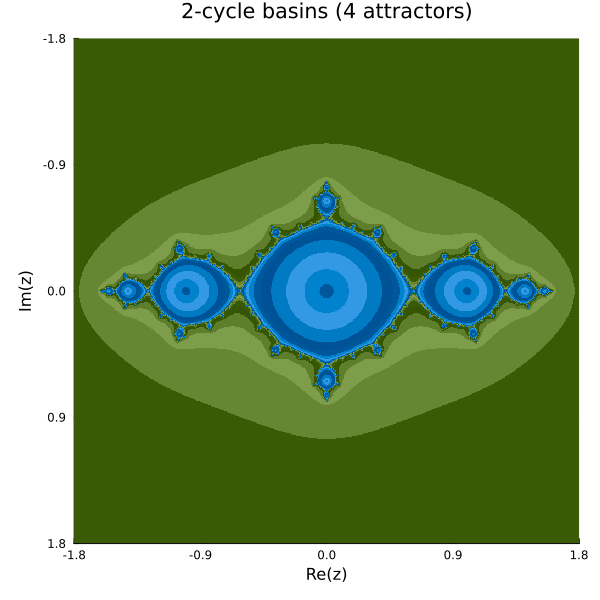
\includegraphics[width=0.65\textwidth]{../figures/pcycle_basilica_2cycle.png}
  \caption{Basin portrait of the 2-cycle of $f_{-1}(z)=z^2-1$ (bas\'ilica).
           Each colour represents the basin of one element of the
           superattracting 2-cycle $\{0,-1\}$; the grey region is the
           basin of $\infty$.}
  \label{fig:basilica_pcycle}
\end{figure}


\subsection{Newton's method for $z^3-1$}

Newton's method $N(z)=\frac{2z^3+1}{3z^2}$ has degree $d=3$.
The Wronskian $W(z)=6z^2\cdot 3z^2 - (2z^3+1)\cdot 6z = 6z(z^3-1)$.
The four critical points are $z=0$ and $z\in\{1,\omega,\bar\omega\}$
where $\omega=e^{2\pi i/3}$.

The three roots of unity are superattracting fixed points of $N$ (Newton
converges quadratically).  The critical point $z=0$ maps to
$N(0)=\infty$; in the second chart $g(w)=3w/(2+w^3)$, $g'(0)=3/2>1$,
so $\infty$ is \emph{repelling} and the orbit of $z=0$ is
\emph{indeterminate}.

The three superattracting fixed points give $P=1$ (see Figure~\ref{fig:newton_z3_pcycle}).

\begin{example}[Newton portrait]
\begin{verbatim}
  num = complex([1.0, 0.0, 0.0, 2.0])
  den = complex([0.0, 0.0, 3.0, 0.0])
  print_critical_orbit_summary(num, den)
  # → 3 superattracting fixed points (p=1), 1 indeterminate
  # → P = 1
  basin_portrait_pcycle(num, den, 1; iter=300, show_plot=true)
\end{verbatim}
\end{example}

\begin{figure}[htbp]
  \centering
  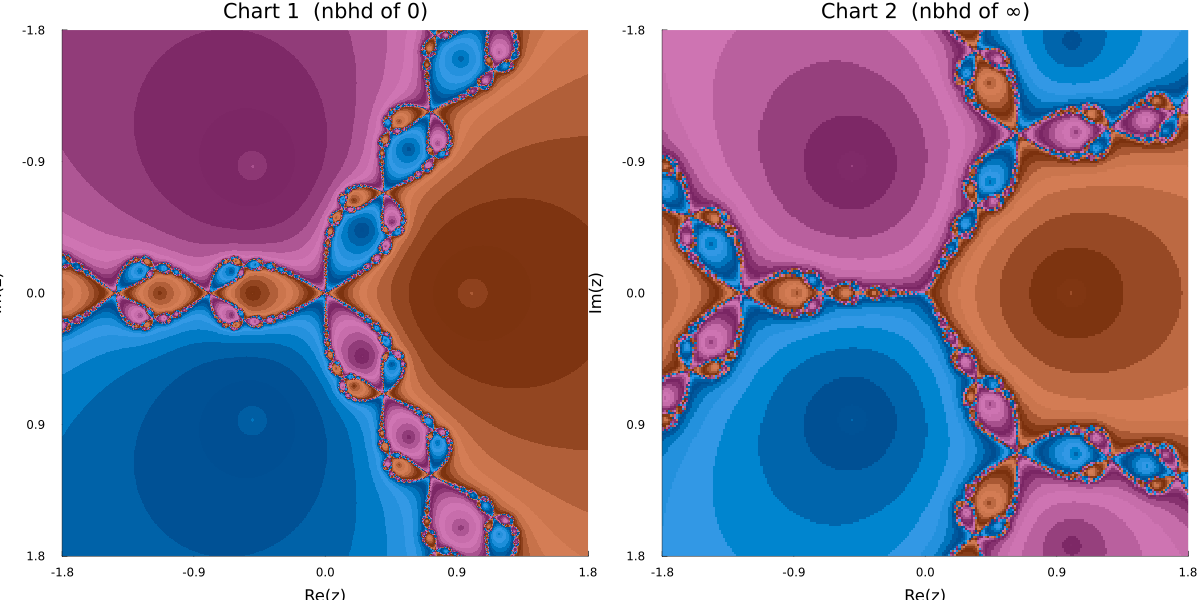
\includegraphics[width=0.90\textwidth]{../figures/pcycle_newton_z3.png}
  \caption{Basin portrait of Newton's method for $z^3-1$ in both affine
           charts of $\Pone$.  Chart~1 (left) shows the neighbourhood of
           the origin; Chart~2 (right) the neighbourhood of $\infty$.
           The three superattracting fixed points (roots of $z^3-1$) each
           attract a connected basin; $\infty$ is repelling.}
  \label{fig:newton_z3_pcycle}
\end{figure}


\subsection{The map $f(z)=z^2$ (superattracting fixed point)}

For $f(z)=z^2$: $W(z)=2z$, unique critical point $z=0$, orbit $0\to 0$.
Since $f'(0)=0$, $c=0$ and $P=1$.  The basin of $0$ is the open unit disc
$\{|z|<1\}$ and the Julia set is the unit circle $\{|z|=1\}$ (see Figure~\ref{fig:z2_fixed}).

\begin{figure}[htbp]
  \centering
  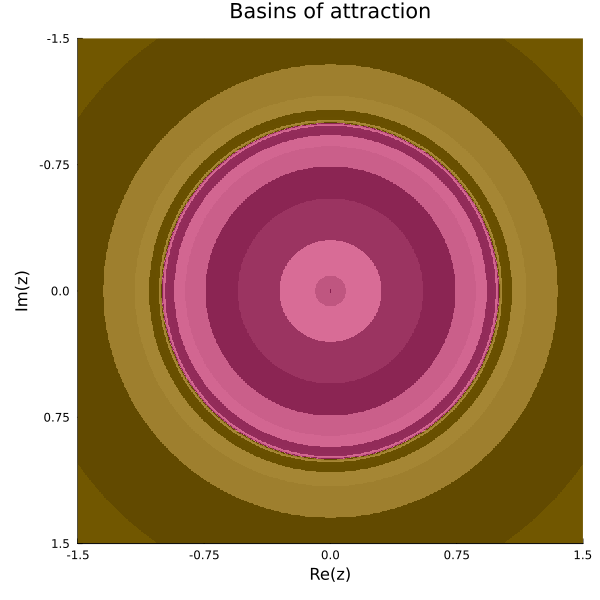
\includegraphics[width=0.55\textwidth]{../figures/pcycle_z2_fixed.png}
  \caption{Basin portrait of $f(z)=z^2$.  The open unit disc $\{|z|<1\}$
           (blue) is the basin of the superattracting fixed point $z=0$;
           the exterior $\{|z|>1\}$ is the basin of $\infty$.
           The unit circle $\{|z|=1\}$ is the Julia set.}
  \label{fig:z2_fixed}
\end{figure}

\subsection{Summary table}

\begin{center}
\begin{tabular}{lcccc}
\toprule
Map & $d$ & $\#$ crit.\ pts & $P$ & Dominant labels\\
\midrule
M\"obius (degree 1)  & 1 & 0  & 0 & --- \\
$f(z)=z^2$         & 2 & 1  & 1 & superattr.\ ($p=1$) \\
$f(z)=z^2-1$       & 2 & 2  & 2 & superattr.\ ($p=2$) + superattr.\ ($p=1$ at $\infty$) \\
Newton $z^3-1$     & 3 & 4  & 1 & 3 superattr.\ ($p=1$) + 1 indet. \\
Halley $z^3-1$     & 5 & 8  & 1 & 3 superattr.\ ($p=1$) \\
\bottomrule
\end{tabular}
\end{center}

%% ===========================================================================
\section{Discussion and open problems}
\label{sec:discussion}
%% ===========================================================================

\subsection{The bound $P$ and its sharpness}

By Corollary~\ref{cor:complete}, the bound $P$ output by
\texttt{max\_attracting\_period} is sharp: there is no attracting cycle
of period $>P$.  However, $P$ is computed via a finite warmup (default
$N_{\mathrm{warm}}=300$), so if the warmup is insufficient for a
slowly-converging attracting cycle, $P$ may be underestimated.
A conservative use of the bound requires checking that the
Lyapunov constant satisfies $c\ll 1$; near a parabolic
parameter where $c\to 1$, the warmup must be increased substantially.

\subsection{Beyond attracting cycles}

The current algorithms detect only attracting and superattracting cycles.
Parabolic cycles ($|\lambda|=1$, $\lambda^q=1$) also attract orbits, but
at polynomial rather than exponential rate; they require a modified
detection scheme based on Fatou coordinates.  Siegel discs and Herman
rings require a different approach (e.g., measuring the autocorrelation
of the orbit to detect irrational rotation numbers).

\subsection{Families and bifurcations}

For a one-parameter family $f_c$ (e.g., $z^2+c$),
the function $c\mapsto P(c)$ records the attracting period.  Its level
sets are the hyperbolic components of the Mandelbrot set
\cite{DouadyHubbard1985}.  An algorithmic study of these boundaries via
\texttt{max\_attracting\_period} applied to a parameter grid is a natural
extension of the present work.

\subsection{Algorithmic complexity and parallelism}

Both algorithms are embarrassingly parallel over grid points
(Algorithm~\ref{alg:basin}) and over critical points
(Algorithm~\ref{alg:critical}).  Julia's threading model and
GPU backends (via \texttt{CUDA.jl}) can accelerate the portrait
computation by several orders of magnitude for high-resolution images.

\subsection{Homogeneous arithmetic and exact computation}

For maps with algebraic coefficients, the Wronskian roots can in principle
be computed exactly (via resultant-based methods).  An exact
implementation would eliminate the deduplication tolerance in
Algorithm~\ref{alg:critical} and give a provably correct critical point
count.

%% ===========================================================================
\section{Conclusions}
\label{sec:conclusions}
%% ===========================================================================

We have presented a self-contained algorithmic framework for the computation
of basins of attraction of $p$-cyclic orbits of rational maps on the Riemann
sphere $\Pone$, based entirely on homogeneous coordinates and the chordal
metric.  The key contributions are:

\begin{enumerate}
  \item A two-chart formula for the spherical derivative $\fsh$
        (Proposition~\ref{prop:sphderiv}) that is correct at all points of
        $\Pone$, including $\infty=[1:0]$, correcting a subtle error in
        naive single-chart implementations (Remark~\ref{rem:chartbug}).

  \item Algorithm~\ref{alg:critical} (\texttt{critical\_orbit\_analysis})
        implementing Fatou's theorem to locate all attracting cycles and
        compute a sharp upper bound $P$ on the maximum attracting period.

  \item Algorithm~\ref{alg:basin} (\texttt{basin\_portrait\_pcycle})
        producing colour-coded basin portraits for any user-specified period
        $p$, with full support for the two-chart global portrait on $\Pone$.

  \item A suite of 94 automated tests in \texttt{RiemannBasins.jl}
        validating the algorithms on the quadratic family, Newton's method,
        and M\"obius transformations.
\end{enumerate}

The combination of Algorithms~\ref{alg:critical} and~\ref{alg:basin} gives a
principled workflow: run Algorithm~\ref{alg:critical} first to determine $P$,
then run Algorithm~\ref{alg:basin} only for $p\leq P$, avoiding unnecessary
computation.

\bigskip
\noindent\textbf{Acknowledgements.}
This work is a continuation of the program
initiated in \cite{Extremiana2019,Alvarez2023}.  Computations were
performed using the Julia language \cite{Julia2017} with the
\texttt{RiemannBasins.jl} package \cite{RiemannBasins}.
L.\,J.\,H.-P.\ acknowledges support from project REGI25/61 of the
Universidad de La Rioja.

%% ===========================================================================
\bibliographystyle{plain}
\bibliography{draft_pcycle_basins}
%% ===========================================================================

\end{document}
